\section{A New Construct and A New Model}
\label{act2.1.2}

\begin{overview}
\textbf{Overview:} A third mechanical energy system -- in addition to \emph{translational kinetic} energy $KE_\text{translational}$ and \emph{gravitational potential} energy $PE_\text{gravity}$ -- is the \emph{spring-mass} energy $PE_\text{spring-mass}$, introduced here in the context of the \SOModel{}.
\end{overview}

\subsection{Oscillating Spring-Mass}

Many physical systems oscillate. The spring-mass system that you are going to examine is one example of many such systems that can be modeled using the \SOModel{}.

\begin{enumerate}
	\item Hang a \unit[200]{g} mass on the spring. The equilibrium position of the mass is the location of the mass when the system is at rest. Use the two-meter stick with the pointer to mark the equilibrium position of the mass. Pull the mass down or push it up \textbf{a few centimeters} and release it. Describe the resulting motion of the mass (e.g., Where is it moving fastest? Where is its speed zero?).
	
	\item Does the resulting motion of the mass depend on whether you started the motion by \emph{lifting the mass up} a certain small distance (try \unit[\about1]{cm}) or by \emph{pulling it down} that same distance from its equilibrium (resting) position?
\end{enumerate}

\WCD

\subsection{Applying the \EnergyInteractionModel{}}
\label{act212.2}

\noindent Work out your responses to the questions below with your small group at the board. Remember that in order to identify an energy system, we need to have an indicator that tells us that the energy system is changing.\\

\noindent Start with the mass pulled down \unit[5]{cm} below its equilibrium position. 

\begin{center}
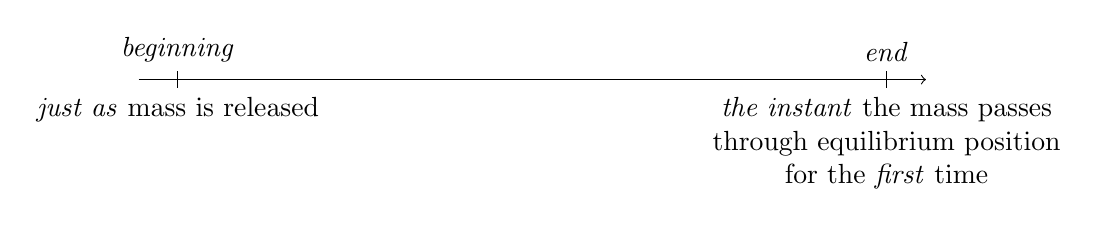
\begin{tikzpicture}
    % draw horizontal line   
    \draw[->] (0,0) -- (10,0);

    % draw vertical lines
    \foreach \x in {0.5,9.5}
      \draw (\x cm,3pt) -- (\x cm,-3pt);

    % draw nodes
    \draw (0.5,0) node[below=3pt] {\emph{just as} mass is released} node[above=3pt] {\emph{beginning}};
    \draw (9.5,0) node[below=3pt, align=center] {\emph{the instant} the mass passes\\through equilibrium position\\for the  \emph{first} time} node[above=3pt] {\emph{end}};
\end{tikzpicture}
\end{center}

\begin{enumerate}
	\item What {\em properties} of the physical system (indicators) changed significantly between the initial and final state?  What energy systems are associated with those indicators?
	\label{act212.2-3}
	
	\item Make a complete \EnergyDiagram{}:
	\label{act212.2-4}
		
	Show the increases and decreases in the energy systems and show the initial and final values of the indicator associated with each energy system -- be as explicit as possible.
	
	\item Write down an algebraic representation of your \EnergyDiagram, expressing energy conservation.

\end{enumerate}

\WCD  

\subsection{Reflecting on the \SOModel{}}

\begin{enumerate}
	\item Do changes in the energy systems you identified depend on the direction that the indicator changed (the sign of the indicator), or only on the magnitude of the indicator?
	
	\item Would the way you modeled this physical system be any different from what you did in your response to \hyperref[act212.2-4]{\ref*{act212.2}\#\ref*{act212.2-4}} if the \textbf{final state} were the instant the mass returned to its equilibrium position the second time, instead of the first?  How about if it were the 200th time?
\end{enumerate}

\WCD